\section{机械系统的控制模型}
机械系统的基本定律是牛顿第二定律$F=ma$。
\subsection{弹簧}
\begin{figure}[!ht]
	\centering
	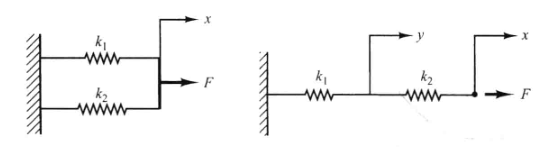
\includegraphics[width=8cm]{figures/3.png}
	\caption{并联与串联弹簧系统}
	\label{3}
\end{figure}

弹簧遵守胡克定律$F=kx$,如\ref{3}所示的并联与串联弹簧系统,其等效劲度系数为

\begin{align*}
k_{eq,parallel}&=k_1+k_2\\
\frac{1}{k_{eq,series}}&=\frac{1}{k_1}+\frac{1}{k_2}
\end{align*}

弹簧可以储贮存势能。

\subsection{阻尼器}

\begin{figure}[!ht]
	\centering
	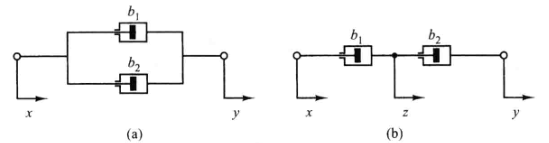
\includegraphics[width=8cm]{figures/4.png}
	\caption{并联与串联阻尼系统}
	\label{4}
\end{figure}

阻尼器可以阻碍相对运动,其提供摩擦力的大小与所连接的两物体间相对速度成正比,即$f=bv$,式中$b$称为粘性摩擦系数。如\ref{4}所示的串联与并联弹簧系统,其等效粘性摩擦系数为

\begin{align*}
b_{eq,parallel}&=b_1+b_2\\
\frac{1}{b_{eq,series}}&=\frac{1}{b_1}+\frac{1}{b_2}
\end{align*}

阻尼器不能贮存动能和势能。

\subsection{质量块}

质量块遵循牛顿第二定律,即$F=ma$。质量块可以贮存动能和势能。